\chapter{User story}
User story zostało przygotowane w formie prezentacji z z dubbingiem głosowym. Slajdy są widoczne na rysunkach
\ref{fig:Slajd1}, \ref{fig:Slajd2}, \ref{fig:Slajd3}, \ref{fig:Slajd4}, \ref{fig:Slajd5}, \ref{fig:Slajd6}, \ref{fig:Slajd7}, \ref{fig:Slajd8}, \ref{fig:Slajd9}.
\begin{figure}[h]
    \centering
    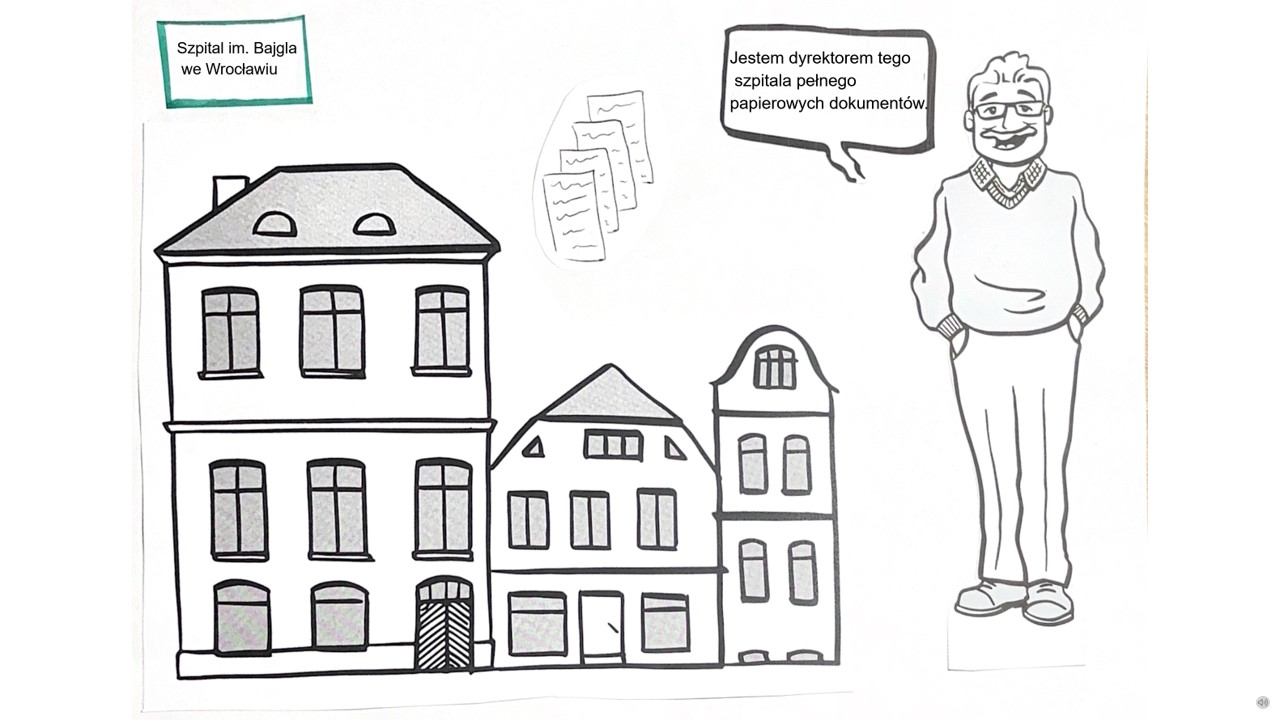
\includegraphics[width=0.8\textwidth]{Grafiki/user story/Slide1.jpg}
    \caption{User story. Slajd 1.}
    \label{fig:Slajd1}
\end{figure}

\begin{figure}[h]
    \centering
    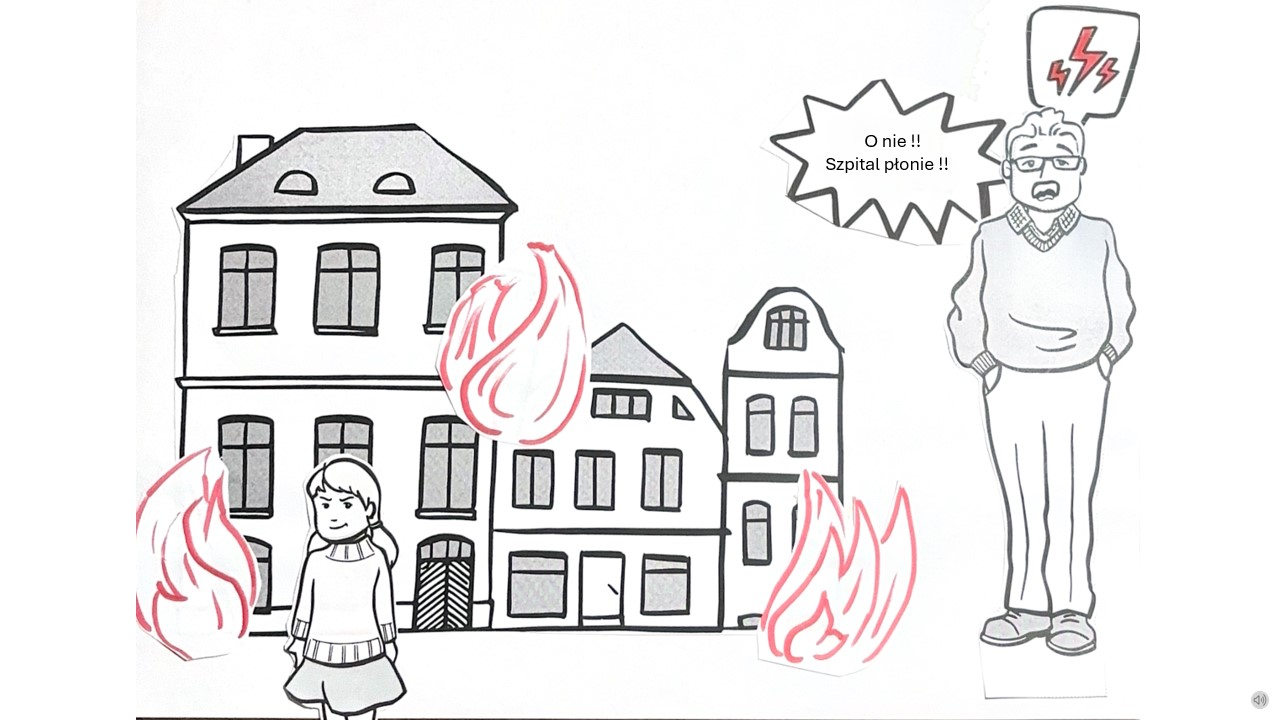
\includegraphics[width=0.8\textwidth]{Grafiki/user story/Slide2.jpg}
    \caption{User story. Slajd 2.}
    \label{fig:Slajd2}
\end{figure}

\begin{figure}[h]
    \centering
    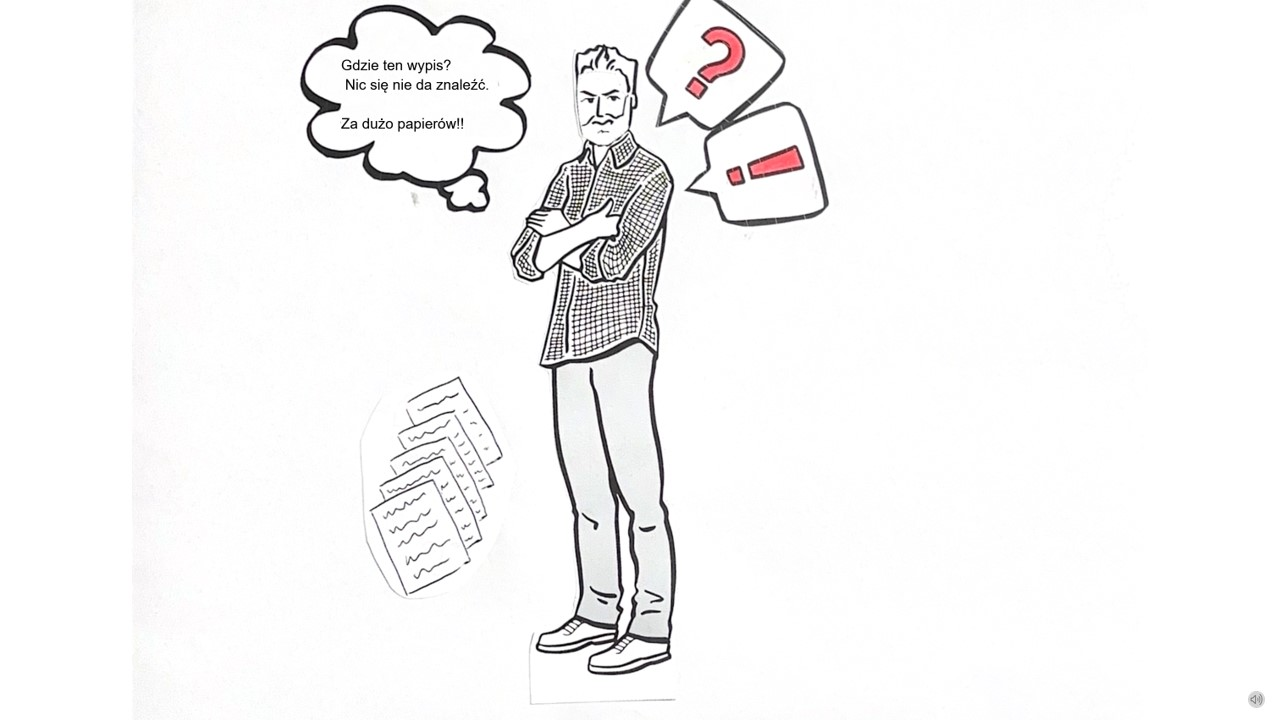
\includegraphics[width=0.8\textwidth]{Grafiki/user story/Slide3.jpg}
    \caption{User story. Slajd 3.}
    \label{fig:Slajd3}
\end{figure}

\begin{figure}[h]
    \centering
    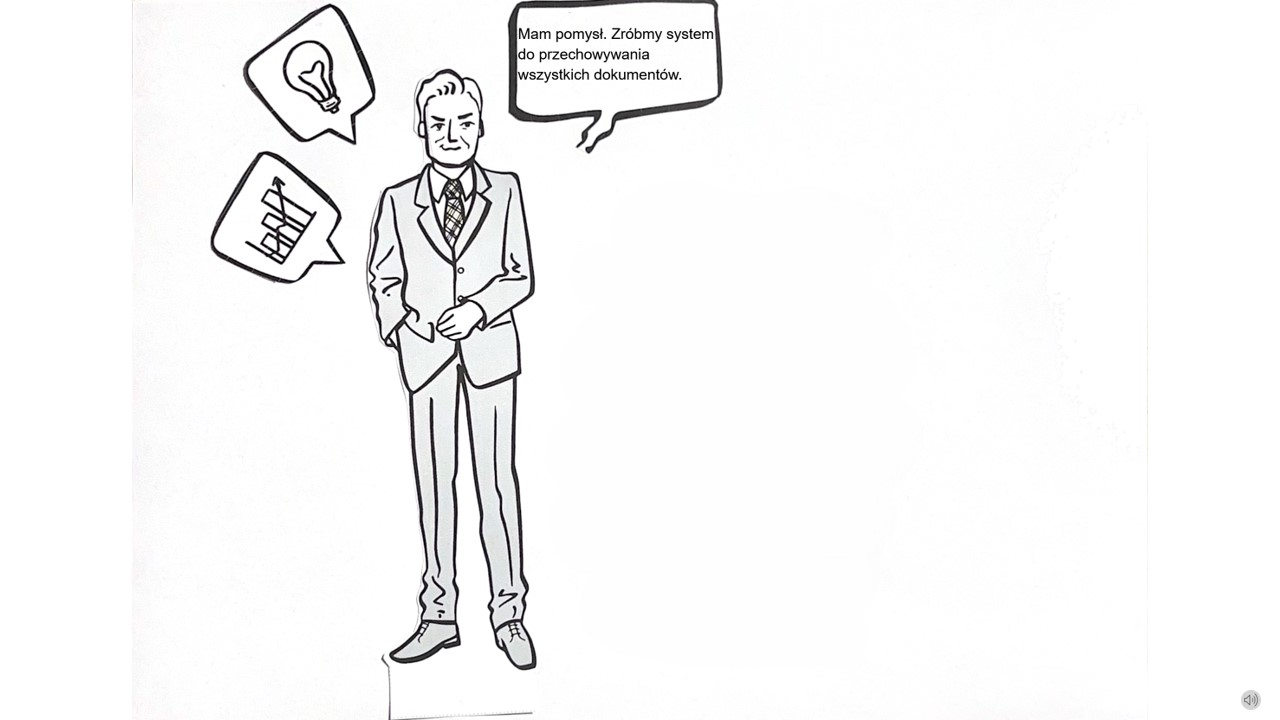
\includegraphics[width=0.8\textwidth]{Grafiki/user story/Slide4.jpg}
    \caption{User story. Slajd 4.}
    \label{fig:Slajd4}
\end{figure}

\begin{figure}[h]
    \centering
    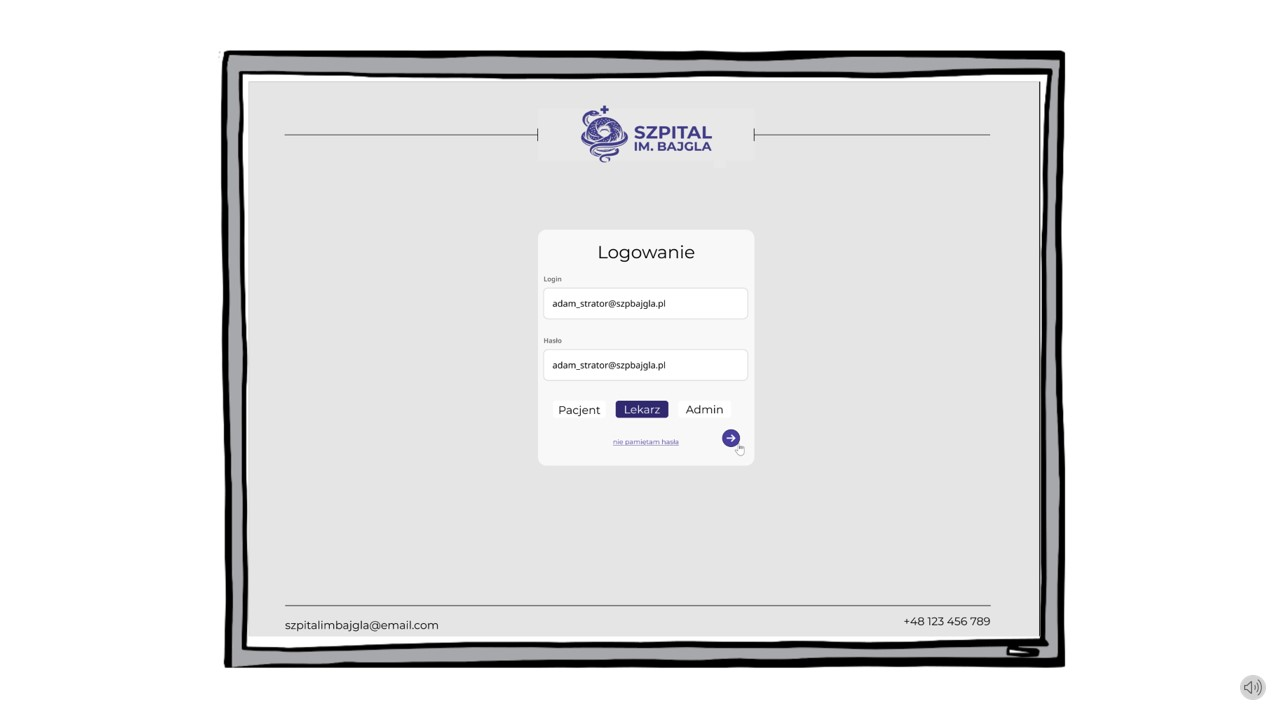
\includegraphics[width=0.8\textwidth]{Grafiki/user story/Slide5.jpg}
    \caption{User story. Slajd 5.}
    \label{fig:Slajd5}
\end{figure}

\begin{figure}[h]
    \centering
    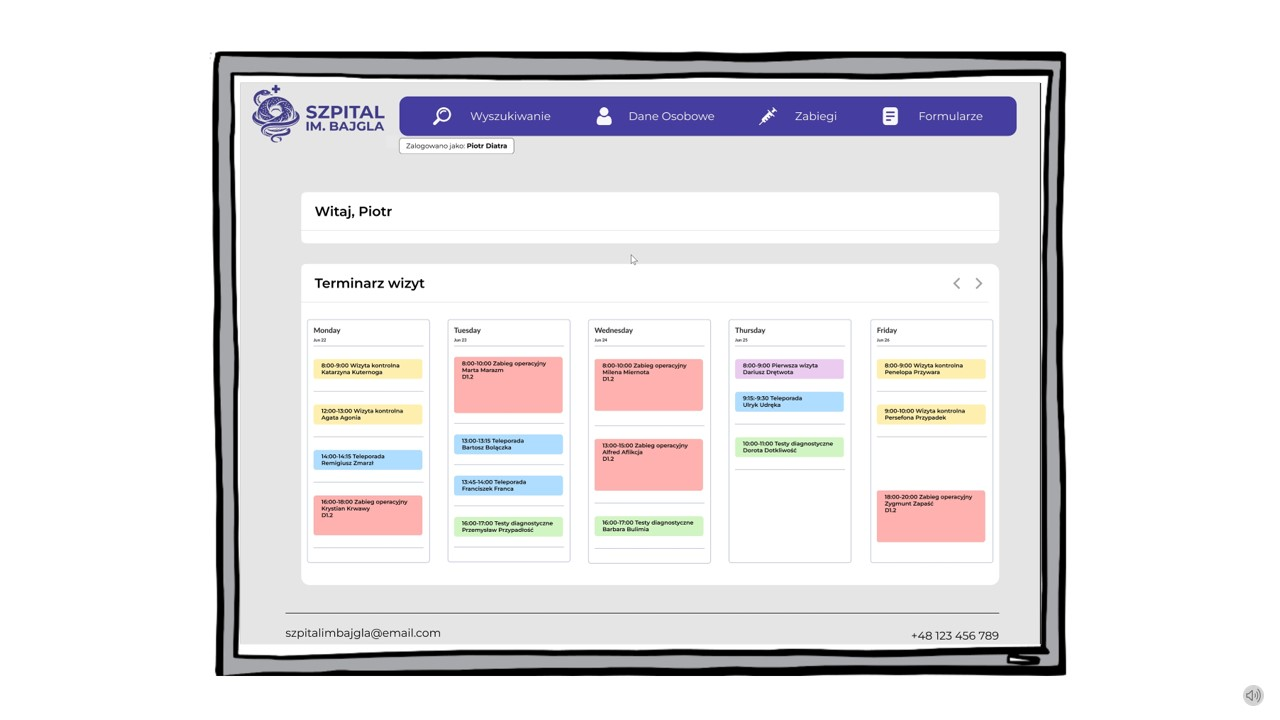
\includegraphics[width=0.8\textwidth]{Grafiki/user story/Slide6.jpg}
    \caption{User story. Slajd 6.}
    \label{fig:Slajd6}
\end{figure}

\begin{figure}[h]
    \centering
    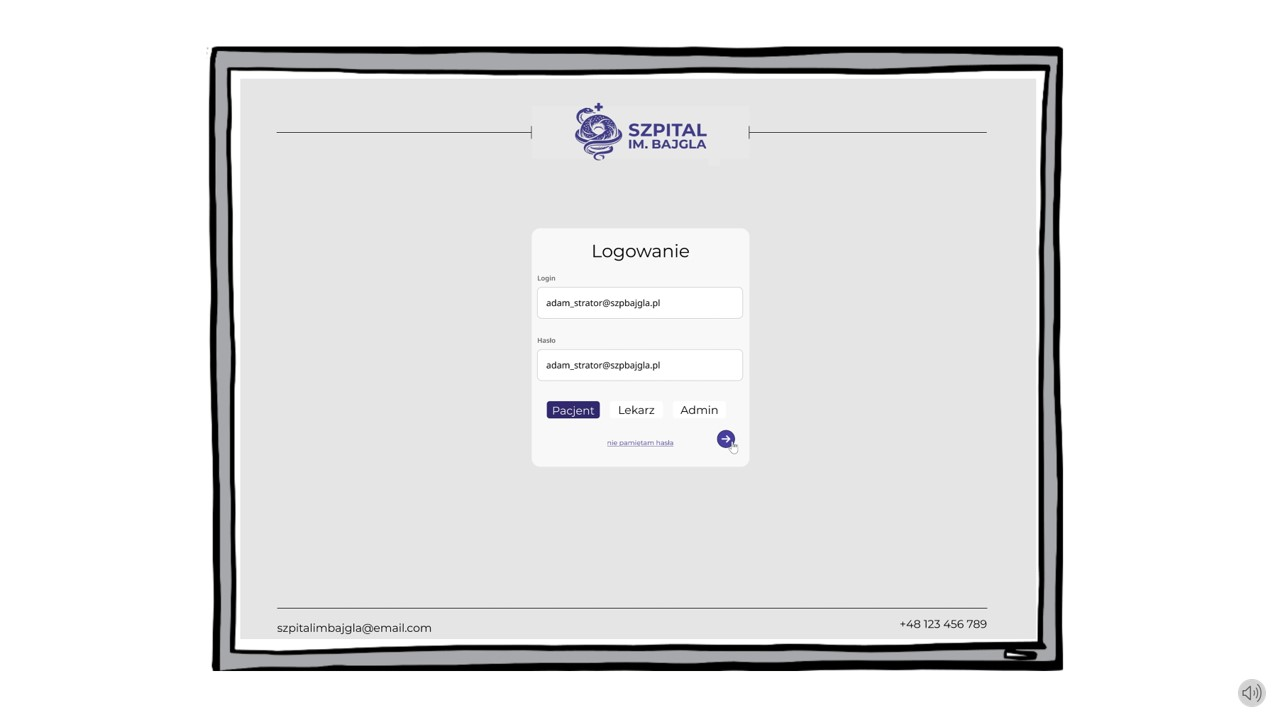
\includegraphics[width=0.8\textwidth]{Grafiki/user story/Slide7.jpg}
    \caption{User story. Slajd 7.}
    \label{fig:Slajd7}
\end{figure}

\begin{figure}[h]
    \centering
    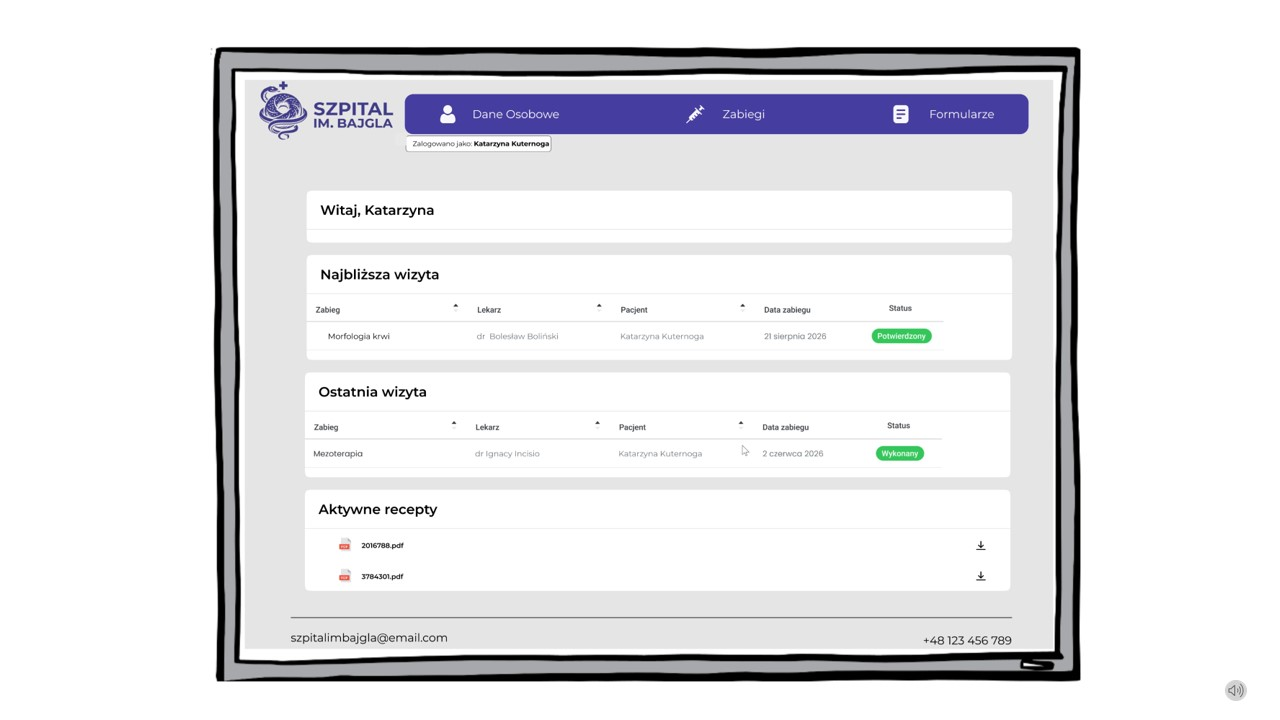
\includegraphics[width=0.8\textwidth]{Grafiki/user story/Slide8.jpg}
    \caption{User story. Slajd 8.}
    \label{fig:Slajd8}
\end{figure}

\begin{figure}[h]
    \centering
    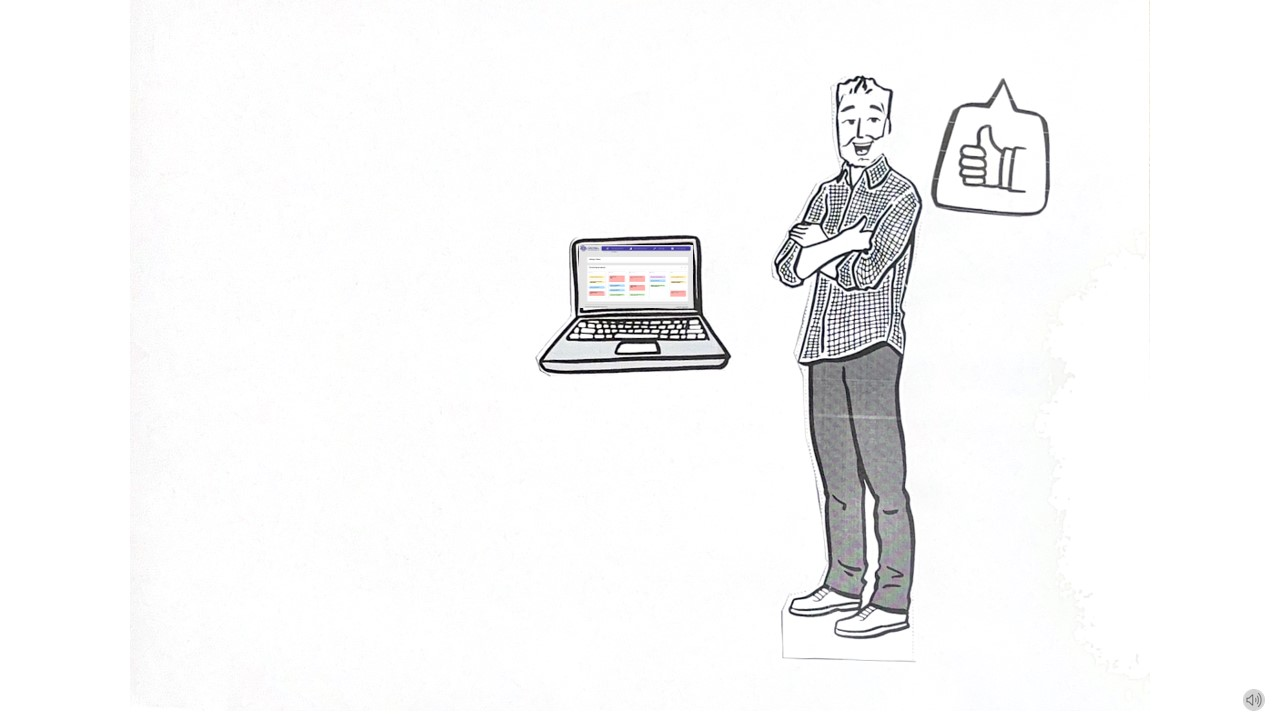
\includegraphics[width=0.8\textwidth]{Grafiki/user story/Slide9.jpg}
    \caption{User story. Slajd 9.}
    \label{fig:Slajd9}
\end{figure}

